\documentclass[aspectratio=169,10pt]{beamer}

\usepackage[T1]{fontenc}
\usepackage{sourcesanspro}
\usepackage{sourcecodepro}
\usepackage{booktabs}
\usepackage{tabularx}
\usepackage{array}
\usepackage{graphicx}
\usepackage{tikz}
\usepackage{pgfplots}
\usepackage{fontawesome5}
\usetikzlibrary{arrows.meta,positioning,fit,calc,shapes.geometric}
\pgfplotsset{compat=1.18}

\definecolor{ArchInk}{HTML}{20252B}
\definecolor{ArchMuted}{HTML}{59636D}
\definecolor{ArchBlue}{HTML}{1F5F7A}
\definecolor{ArchBlueLight}{HTML}{EAF3F7}
\definecolor{ArchGreen}{HTML}{3D7A57}
\definecolor{ArchGreenLight}{HTML}{EDF6EF}
\definecolor{ArchRed}{HTML}{A42A38}
\definecolor{ArchRedLight}{HTML}{FAECEE}
\definecolor{ArchGold}{HTML}{B47A18}
\definecolor{ArchGoldLight}{HTML}{FBF3E3}
\definecolor{ArchLine}{HTML}{C8D1D8}
\definecolor{ArchPanel}{HTML}{F6F8F9}

\setbeamercolor{normal text}{fg=ArchInk,bg=white}
\setbeamercolor{structure}{fg=ArchBlue}
\setbeamercolor{frametitle}{fg=ArchInk,bg=white}
\setbeamercolor{alerted text}{fg=ArchRed}
\setbeamerfont{title}{size=\fontsize{26}{30}\selectfont,series=\bfseries}
\setbeamerfont{subtitle}{size=\fontsize{13}{16}\selectfont}
\setbeamerfont{frametitle}{size=\fontsize{18}{22}\selectfont,series=\bfseries}
\setbeamerfont{footline}{size=\fontsize{6.8}{8}\selectfont}
\setbeamertemplate{navigation symbols}{}
\setbeamertemplate{itemize item}{\color{ArchBlue}\small$\blacksquare$}
\setbeamertemplate{itemize subitem}{\color{ArchMuted}\scriptsize$\blacktriangleright$}
\setbeamersize{text margin left=0.55cm,text margin right=0.55cm}

\setbeamertemplate{frametitle}{%
  \nointerlineskip
  \begin{beamercolorbox}[wd=\paperwidth,ht=0.72cm,dp=0.13cm,leftskip=0.58cm,rightskip=0.58cm]{frametitle}
    \usebeamerfont{frametitle}\insertframetitle
  \end{beamercolorbox}
  \vspace{-0.08cm}
  \hspace{0.58cm}\color{ArchBlue}\rule{1.15cm}{0.75pt}\color{ArchLine}\rule{\dimexpr\paperwidth-2.31cm\relax}{0.35pt}
  \vspace{0.12cm}
}

\setbeamertemplate{footline}{%
  \begin{beamercolorbox}[wd=\paperwidth,ht=0.45cm,dp=0.2cm]{footline}
    \hspace{0.58cm}\color{ArchMuted}\insertshorttitle\hfill\insertframenumber\hspace{0.58cm}
  \end{beamercolorbox}
}

\title{\textcolor{ArchBlue}{Architecture 2.0:} The XR Lighthouse Workshop}
\subtitle{Translating AI-Assisted Principles into Verifiable Hardware Practice}
\author{}
\date{}

\begin{document}

\begin{frame}[plain]
  \vspace{1.5cm}
  \usebeamerfont{title}\inserttitle\par
  \vspace{0.25cm}
  \usebeamerfont{subtitle}\textcolor{ArchMuted}{\insertsubtitle}\par
  \vspace{1.5cm}

  \small\textcolor{ArchInk}{\textbf{Objective:}} Navigate the physical constraints, verification bottlenecks, and proprietary data moats of AI-assisted chip design through 12 interactive Colab notebooks.
\end{frame}

\begin{frame}{The XR Lighthouse Benchmark}
  \textbf{We are building a low-power mobile XR subsystem.}

  \vspace{0.3cm}
  This is our \textit{SWE-bench for hardware}. It imposes strict constraints:
  \begin{itemize}
    \item 64-bit RISC-V compute core
    \item 3W thermal budget
    \item 15ms latency limit
    \item Tight die area constraints
  \end{itemize}

  \vspace{0.3cm}
  \begin{center}
    \fcolorbox{ArchLine}{ArchPanel}{
      \parbox{0.9\textwidth}{
        \small
        \textbf{The Challenge:} Static dictionaries are not benchmarks.
        You will interact with a parameterized mathematical model where changing the L2 cache size
        has \textcolor{ArchRed}{\textbf{non-linear}} secondary effects on off-chip traffic, power, and latency.
      }
    }
  \end{center}
\end{frame}

\begin{frame}{IP Provenance and Viral Contamination}
  \textbf{Lab 01: The Danger of Raw LLM Regurgitation}

  \vspace{0.3cm}
  When LLMs output raw hardware code (e.g., Verilog/Chisel), they often regurgitate snippets from their training data.

  \vspace{0.4cm}
  \begin{itemize}
    \item \textbf{GPLv3 / Viral Licenses:} Legally compromises the entire proprietary SoC.
    \item \textbf{Unknown Provenance:} Presents a critical risk for tapeout compliance.
    \item \textbf{The Solution:} We must enforce strict context wiping and \textit{IP Isolation} when transferring generated artifacts to proprietary physical validation.
  \end{itemize}
\end{frame}

\begin{frame}{Navigating Proprietary Data Moats}
  \textbf{Lab 02: Open-Source Agility vs. Physical Realities}

  \vspace{0.3cm}
  Why do AI-generated architectures frequently fail in the final mile?

  \vspace{0.2cm}
  \begin{itemize}
    \item \textbf{Open-Source Tools (e.g., SCALE-Sim):} Fast, mathematically deterministic, great for high-volume upstream screening.
    \item \textbf{The Data Moat:} Closely guarded physical PPA libraries (Power, Performance, Area) held by incumbent foundries.
  \end{itemize}

  \vspace{0.2cm}
  \textbf{The Gap:} A design deemed "optimal" by a linear open-source estimator will catastrophically fail at the proprietary foundry due to non-linear physical constraints (e.g., wire delay congestion limits).
\end{frame}

\begin{frame}{Surviving the Verification Bottleneck}
  \textbf{Lab 05: Structural Pruning Proxies}

  \vspace{0.3cm}
  Flooding a narrow, expensive EDA pipeline with cheap AI-generated candidates leads to O(N) verification explosions.

  \vspace{0.4cm}
  \begin{center}
  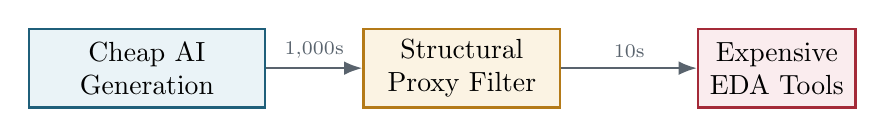
\begin{tikzpicture}[x=1cm,y=1cm]
    % Generation
    \node[draw=ArchBlue, fill=ArchBlueLight, thick, minimum width=3cm, minimum height=1cm, align=center] (gen) at (0,0) {Cheap AI\\Generation};

    % Proxy
    \node[draw=ArchGold, fill=ArchGoldLight, thick, minimum width=2.5cm, minimum height=1cm, align=center] (proxy) at (4,0) {Structural\\Proxy Filter};

    % Verification
    \node[draw=ArchRed, fill=ArchRedLight, thick, minimum width=2cm, minimum height=1cm, align=center] (ver) at (8,0) {Expensive\\EDA Tools};

    \draw[-Latex, thick, ArchMuted] (gen) -- node[above] {\scriptsize 1,000s} (proxy);
    \draw[-Latex, thick, ArchMuted] (proxy) -- node[above] {\scriptsize 10s} (ver);
  \end{tikzpicture}
  \end{center}

  \vspace{0.4cm}
  \textbf{The Fix:} We build an imperfect but fast heuristic proxy that prunes failing heuristics in milliseconds, saving hours of simulator time.
\end{frame}

\begin{frame}{Workshop Execution}
  \textbf{Let's dive in.}

  \vspace{0.3cm}
  \begin{itemize}
    \item Open Google Colab.
    \item Navigate to \texttt{Lab\_00\_Introduction\_and\_Setup.ipynb}.
    \item Follow the 12-lab sequence to evaluate, design, verify, and legally secure a hardware architecture.
  \end{itemize}

  \vspace{1cm}
  \begin{center}
    \textcolor{ArchBlue}{\Large \faLaptopCode} \hspace{0.2cm} \textbf{Ready to start.}
  \end{center}
\end{frame}

\end{document}
